\documentclass[a4paper, 12pt]{article}
\usepackage[utf8]{inputenc}

\usepackage[a4paper,top=1.3cm,bottom=2cm,left=1.5cm,right=1.5cm,marginparwidth=0.75cm]{geometry}
\usepackage{cmap}				
\usepackage{mathtext} 				
\usepackage[T2A]{fontenc}			
\usepackage[utf8]{inputenc}			
\usepackage[english,russian]{babel}	
\usepackage{multirow}
\usepackage{mathtools}
\mathtoolsset{showonlyrefs=true}

\usepackage{graphicx}
\usepackage{wrapfig}
\usepackage{tabularx}
\usepackage{caption}

\title{2.1.3-theory}
\author{Влад Черниенко}
\date{March 2022}


\begin{document}

    \begin{titlepage}
    
        \begin{center}
            {\large МОСКОВСКИЙ ФИЗИКО-ТЕХНИЧЕСКИЙ ИНСТИТУТ (НАЦИОНАЛЬНЫЙ ИССЛЕДОВАТЕЛЬСКИЙ УНИВЕРСИТЕТ)}
        \end{center}
        \begin{center}
            {\large Фихтех-школа радиотехники и компьютерных технологий}
        \end{center}
        
        \vspace{4.5cm}
        
        {\huge
            \begin{center}
                {\bf Лабораторная работа 2.5.1}\\
                Измерение коэффициента поверхностного натяжения жидкости
            \end{center}
        }
        
        \vspace{11cm}
        
        \begin{flushright}
            {\LARGE Автор: \\ Черниенко Владислав Антонович \\ \vspace{0.2cm} Группа Б01-110}
        \end{flushright}
        
    \end{titlepage}
    
    
    \noindent {\bf Цель работы:} 1) измерение температурной зависимости  коэффициента поверхностного натяжения дистиллированной воды с использованием известного коэффициента поверхностного натяжения спирта; 2) определение полной поверхностной энергии  и теплоты, необходимой для изотермического образования единицы поверхности жидкости при различной температуре.\\
    
    \noindent {\bf В работе используются:} прибор Ребиндера с термостатом и микроманометром; исследуемые жидкости; стаканы.\\
    
    \begin{flushleft}
        {\Large {\bf Теоретические сведения}}
    \end{flushleft}
    
    Наличие поверхностного слоя приводит к различию давлений по разные стороны от искривленной границы раздела двух сред. Для сферического пузырька с воздухом внутри жидкости избыточное давление даётся формулой Лапласа:
    \begin{equation}
        \Delta P = P_{внутри} - P_{снаружи} = \frac{2 \sigma}{r},
        \label{first}
    \end{equation}
    где $\sigma$ – коэффициент поверхностного натяжения, $P_{внутри}$ и $P_{снаружи}$ – давление внутри пузырька и снаружи, $r$ – радиус кривизны поверхности раздела двух фаз. Эта формула лежит в основе предлагаемого метода определения коэффициента поверхностного натяжения жидкости. Измеряется давление $\Delta P$, необходимое для выталкивания в жидкость пузырька воздуха.
    
    \begin{figure}[ht]
        \centering
        \captionsetup{justification=centering, margin=2cm}
        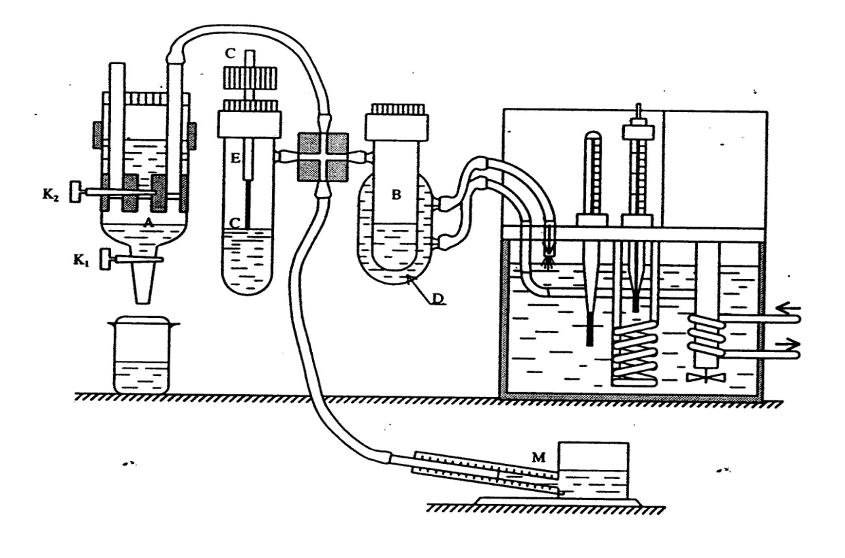
\includegraphics[width=0.8\linewidth]{images/ust.png}
        \caption{Схема установки для измерения температурной зависимости коэффициента поверхностного натяжения}
        \label{pic1}
    \end{figure}
    
    \begin{flushleft}
        {\Large {\bf Экспериментальная установка}}
    \end{flushleft}
    
    Исследуемая жидкость (дистиллированная вода) наливается в сосуд (колбу) $B$ (рис. \ref{pic1}). Тестовая жидкость  (этиловый спирт) наливается  в сосуд $E$.  При измерениях  колбы герметично закрываются  пробками.   Через одну из двух пробок  проходит полая металлическая игла $C$. Этой пробкой закрывается сосуд, в котором  проводятся измерения. Верхний конец иглы открыт в атмосферу, а нижний погружен в жидкость. Другой сосуд герметично закрывается второй пробкой. При создании достаточного  разряжения воздуха в колбе с иглой пузырьки воздуха начинают пробулькивать через жидкость. Поверхностное натяжение можно определить по величине разряжения $\Delta P$ \eqref{first}, необходимого для прохождения пузырьков (при известном радиусе иглы).
    
    Разряжение в системе создается с помощью аспиратора $A$. Кран $K_2$ разделяет две полости аспиратора. Верхняя полость при закрытом кране $K_2$ заполняется водой. Затем кран $K_2$ открывают и заполняют водой нижнюю полость аспиратора. Разряжение воздуха создается в нижней полости при открывании крана $K_1$, когда вода вытекает из неё по каплям. В колбах $B$ и $C$, соединённых трубками с нижней полостью аспиратора, создается такое же пониженное давление. Разность давлений в полостях с разряженным воздухом и атмосферой измеряется спиртовым микроманометром. Для стабилизации температуры исследуемой жидкости через рубашку $D$ колбы $B$ непрерывно прогоняется вода из термостата.
    
    Обычно кончик иглы лишь касается поверхности жидкости, чтобы исключить влияние гидростатического давления столба жидкости. Однако при измерении температурной зависимости коэффициента поверхностного натяжения возникает ряд сложностей. Во-первых, большая теплопроводность металлической трубки приводит к тому, что температура на конце трубки заметно ниже, чем в глубине жидкости. Во-вторых, тепловое расширение поднимает уровень жидкости при увеличении температуры.
    
    Обе погрешности можно устранить, погрузив кончик трубки до самого дна. Полное давление, измеренное при этом микроманометром, $P = \Delta P + \rho g h$. Заметим, что $\rho g h$ от температуры практически не зависит, так как подъём уровня жидкости компенсируется уменьшением её плотности (произведение $\rho h$ определяется массой всей жидкости и поэтому постоянно). Величину $\rho g h$ следует измерить двумя способами. Во-первых, замерить величину $P_1 = \Delta P'$, когда кончик трубки только касается поверхности жидкости. Затем при этой же температуре опустить иглу до дна и замерить $P_2 = \rho g h + \Delta P''$ ($\Delta P'$, $\Delta P''$ – давление Лапласа). Из-за несжимаемости жидкости можно положить $\Delta P' = \Delta P''$ и тогда $\rho g h = P_2 - P_1$. Во-вторых, при измерениях $P_1$ и $P_2$ замерить линейкой глубину погружения иглы $h$. Это можно сделать, замеряя расстояние между верхним концом иглы и любой неподвижной частью прибора при положении иглы на поверхности и в глубине колбы.\\
    
    \begin{flushleft}
        {\Large {\bf Ход работы/Обработка результатов измерений}}
    \end{flushleft}
    
    \begin{enumerate}
    
        \item[1.] Откроем кран $K_1$ и подберём частоту падения капель из аспиратора так, чтобы максимальное давление манометра не зависело от этой частоты.
        
        \item[2.] Измерим максимальное давление при пробулькивании пузырьков воздуха через спирт. Давление будем считать по следующей формуле:
        \begin{equation}
            \Delta P_{сп} = 0,2 \cdot \rho g h_{сп},
            \label{eq2}
        \end{equation}
        где $\rho$ — плотность спирта ($\rho_{сп} = 809,5 \text{ } кг/м^3$), $g$ — ускорение свободного падения ($g = 9,80665 \text{ } м/с^2$), $h_{сп}$ — показание шкалы микроманометра.
        
        По формуле \eqref{first} найдём диаметр иглы:
        \begin{equation}
            d = \frac{4 \sigma_{сп}}{\Delta P_{сп}} = \frac{4 \sigma_{сп}}{0,2 \cdot \rho g h_{сп}}.
            \label{eq3}
        \end{equation}
        Значение коэффициента поверхностного натяжения спирта возьмём табличное: $\sigma_{спирт} = 22,75 \cdot 10^{-3} \text{ } Н/м$.
        
        Рассчитаем погрешности измерений. Для уменьшения случайной погрешности проведём $n = 5$ измерений. Результаты будем заносить в табл. \ref{table1}. Класс точности микроманометра равен 1. Значит приборная погрешность $\sigma_h^{приб} = 3 \text{ } мм$. Случайную погрешность $\sigma_h^{случ}$ рассчитаем по следующей формуле:
        \begin{equation}
            \sigma_h^{случ} = \sqrt{\frac{1}{n (n - 1)} \sum_{i = 1}^n (h_i - \langle h \rangle)^2},
        \end{equation}
        тогда
        \begin{equation}
            \sigma_h = \sqrt{(\sigma_h^{приб})^2 + (\sigma_h^{случ})^2}.
        \end{equation}
        
        \begin{table}[ht]
            \centering
            \begin{tabular}{|c|c|c|c|c|c|}
                \hline
                $h_{сп}, \text{ } мм$ & 39 & 40 & 40 & 41 & 39 \\
                \hline
                $\langle h_{сп} \rangle, \text{ } мм$ & 39,8 & $\sigma_{h_{сп}}, \text{ } мм$ & 3,0 & $\varepsilon_{h_{сп}}, \text{ } \%$ & 7,6 \\
                \hline
            \end{tabular}
            \caption{Значения шкалы микроманометра при опускании иглы в спирт}
            \label{table1}
        \end{table}
        
        Из \eqref{eq3} видно, что $\varepsilon_d = \varepsilon_{h_{сп}}$. В итоге получаем
        \begin{equation}
            d = (1,44 \pm 0,11) \text{ } мм.
        \end{equation}
        
        Далее измерим диаметр иглы с помощью микроскопа. Приборная погрешность микроскопа: $\sigma_d = 0,05 \text{ } мм$. Получим
        \begin{equation}
            d = (1,23 \pm 0,05) \text{ } мм.
        \end{equation}
        
        \item[3.] Перенесём предварительно промытую и просушенную от спирта иглу в колбу с дистиллированной водой. Установим иглу в положении, в котором она слегка касается поверхности воды. Предварительно заполним аспиратор водой почти доверху. Отрегулируем скорость поднятия уровня спирта в манометре. Далее измерим расстояние между верхним концом иглы и неподвижной частью прибора линейкой: $h_1 = (2,10 \pm 0,05) \text{ } см$. 
        
        Измерим максимальное давление при пробулькивании пузырьков воздуха через воду, результаты будем заносить в табл. \ref{table2}.
        
        \begin{table}[ht]
            \centering
            \begin{tabular}{|c|c|c|c|c|c|}
                \hline
                $h_{в_1}, \text{ } мм$ & 110 & 112 & 112 & 111 & 112 \\
                \hline
                $\langle h_{в_1} \rangle, \text{ } мм$ & 111,4 & $\sigma_{h_{в_1}}, \text{ } мм$ & 3,0 & $\varepsilon_{h_{в_1}}, \text{ } \%$ & 2,7 \\
                \hline
            \end{tabular}
            \caption{Значения шкалы микроманометра при опускании иглы в воду}
            \label{table2}
        \end{table}
        
        По формуле: $h_{сп} / \sigma_{сп} = h_в / \sigma_в$ найдём $\sigma_в$
        \begin{equation}
            \sigma_в = \sigma_{сп} \cdot \frac{h_в}{h_{сп}},
        \end{equation}
        погрешность данной величины рассчитаем по следующей формуле:
        \begin{equation}
            \varepsilon_{\sigma_в} = \sqrt{\varepsilon_{h_{сп}}^2 + \varepsilon_{h_в}^2}.
        \end{equation}
        В итоге получим
        \begin{equation}
            \sigma_в = (6,4 \pm 0,5) \cdot 10^{-2} \text{ } Н/м.
        \end{equation}
        
        По формуле \eqref{eq2} найдём $P_1$:
        \begin{equation}
            P_1 = 0,2 \cdot \rho g h_{в_1},
        \end{equation}
        погрешность посчитаем по следующей формуле:
        \begin{equation}
            \varepsilon_{P_1} = \varepsilon_h.
        \end{equation}
        В итоге получим
        \begin{equation}
            P_1 = (1,76 \pm 0,05) \cdot 10^2 \text{ } Па.
        \end{equation}
        
        \item[4.] Будем опускать иглу до того момента, пока не услышым характерный щелчок прибора. Измерим расстояние между верхним концом иглы и неподвижной частью прибора линейкой (как в п. 3): $h_2 = (0,65 \pm 0,05) \text{ } см$.
        
        Измерим максимальное давление в пузырьках. Результаты занесём в табл. \ref{table3}.
        
        \begin{table}[ht]
            \centering
            \begin{tabular}{|c|c|c|c|c|c|}
                \hline
                $h_{в_{2}}, \text{ } мм$ & 178 & 179 & 181 & 181 & 180 \\
                \hline
                $\langle h_{в_2} \rangle, \text{ } мм$ & 179,8 & $\sigma_{h_{в_2}}, \text{ } мм$ & 3,1 & $\varepsilon_{h_{в_1}}, \text{ } \%$ & 1,7 \\
                \hline
            \end{tabular}
            \caption{Значения шкалы микроманометра при погружении иглы в воду}
            \label{table3}
        \end{table}
        
        Рассчитаем давление $P_2$ по формуле: $P_2 = 0,2 \cdot \rho g h_{в_2}$. Погрешность данной величины: $\varepsilon_{P_2} = \varepsilon_h$. В итоге получим
        \begin{equation}
            P_2 = (2,85 \pm 0,05) \cdot 10^2 \text{ } Па.
        \end{equation}
        
        Рассчитаем $\Delta h$ через разность давлений $P_1$ и $P_2$ по формуле:
        \begin{equation}
            \Delta h = \frac{P_2 - P_1}{\rho_в g}.
        \end{equation}
        Погрешность $\Delta h$ оценим по следующим формулам:
        \begin{equation}
            \varepsilon_{\Delta h} = \varepsilon_{\Delta P},
        \end{equation}
        \begin{equation}
            \sigma_{\Delta P} = \sqrt{\sigma_{P_1}^2 + \sigma_{P_2}^2}.
        \end{equation}
        В итоге получим
        \begin{equation}
            \Delta h = (1,11 \pm 0,07) \text{ } см.
        \end{equation}
        
        При прямом измерении $\Delta h$ получим значение
        \begin{equation}
            \Delta h = (1,45 \pm 0,07) \text{ } см.
        \end{equation}
        
        \item[5.] Снимем температурную зависимость $\sigma (T)$ дистиллированной воды. Для этого включим термостат и подождём, пока нужная нам температура не стабилизируется. Затем измерим давление. Измерять давление будем при температурах от комнатной до $60^{\circ} \text{C}$ с шагом в $3^\circ \text{C}$. Давление будем рассчитывать по формуле \eqref{eq2}, затем коэффициент поверхностного натяжения будем считать по формуле:
        \begin{equation}
            \sigma = \frac{\Delta P \cdot d}{4} = \frac{(0,2 \cdot \rho g h - \rho_в g \cdot \Delta h) \cdot d}{4}.
        \end{equation}
        Построим график зависимости $\sigma (T)$. Результат представим на рис. \ref{pic2}.
        
        По данному графику найдём значение коэффициента наклона прямой $d \sigma/d T$ и оценим его погрешность. Погрешность будем рассчитывать по следующим формулам:
        \begin{equation}
            \varepsilon_{d\sigma/dT}^{приб} = \sqrt{\varepsilon_{\Delta P}^2 + \varepsilon_d^2},
        \end{equation}
        \begin{equation}
            \sigma_{\Delta P} = \sqrt{(0,2 \cdot \rho g \cdot \sigma_h)^2 + (\rho_в g \cdot \sigma_{\Delta h})^2},
        \end{equation}
        \begin{equation}
            \sigma_{d\sigma/dT}^{случ} = \frac{1}{\sqrt{n}} \sqrt{\frac{\langle \sigma^2 \rangle - \langle \sigma \rangle^2}{\langle T^2 \rangle - \langle T \rangle^2} - \left( \frac{d\sigma}{dT} \right)^2},
        \end{equation}
        \begin{equation}
            \sigma_{d\sigma/dT} = \sqrt{(\sigma_{d\sigma/dT}^{приб})^2 + (\sigma_{d\sigma/dT}^{случ})^2}.
        \end{equation}
        В итоге получаем
        \begin{equation}
            \frac{d\sigma}{dT} = (-0,99 \pm 0,12) \cdot 10^{-4} \text{ } Н/(м \cdot К).
        \end{equation}
        
        \item[6.] Построим графики зависимости от температуры: 1) единицы поверхности жидкости $q(T) = -T \cdot \frac{d\sigma}{dT}$; 2) поверхностной энергии $U$ единицы площади $F$: $\frac{U}{F}(T) = (\sigma - T \cdot \frac{d\sigma}{dT})$. Результаты представим на рис. \ref{pic3} и \ref{pic4}.
    
        \newpage
                
        \begin{figure}[ht]
            \centering
            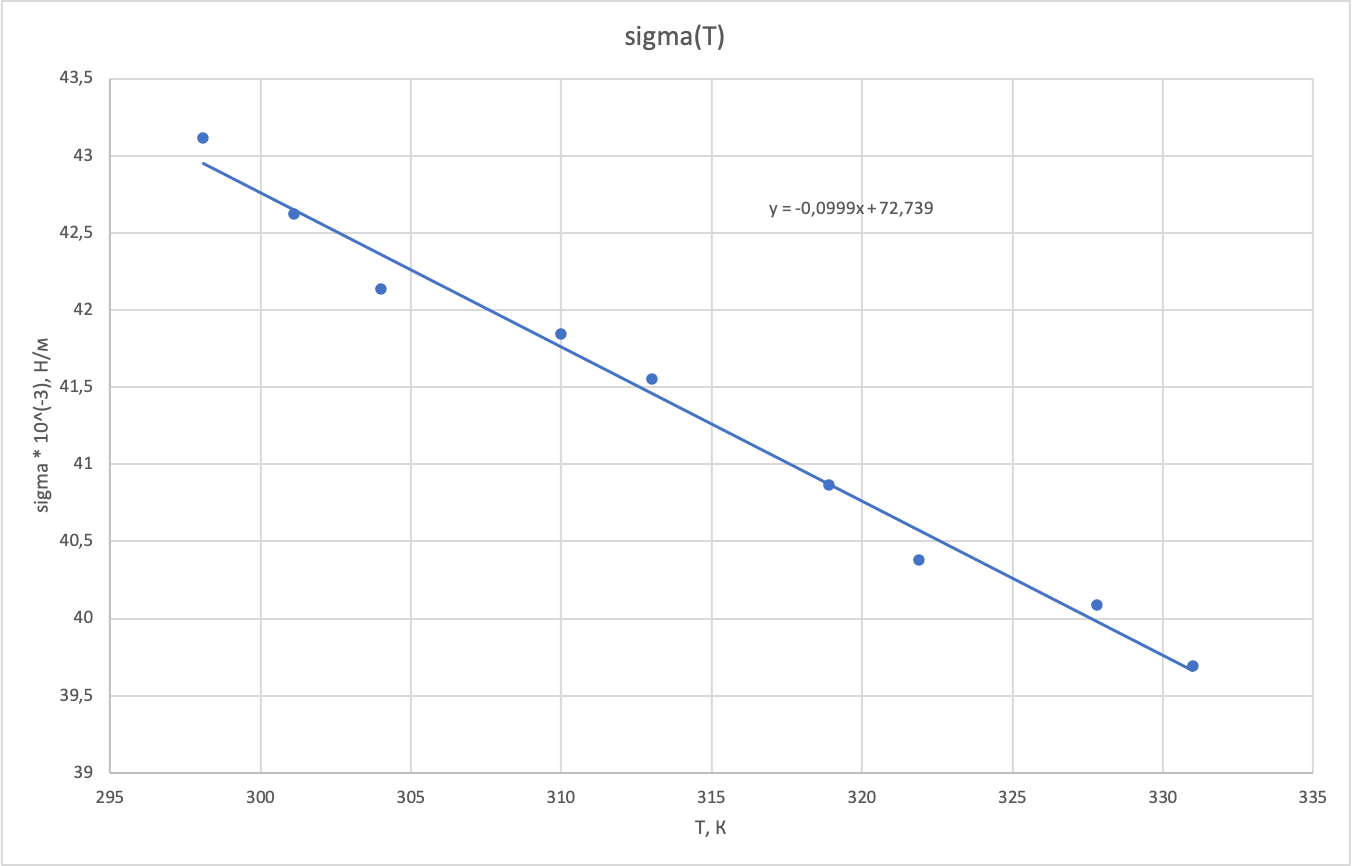
\includegraphics[width=0.75\linewidth]{images/sigma(T).png}
            \caption{График зависимости $\sigma (T)$}
            \label{pic2}
        \end{figure}
        
        \vspace{2cm}
        
        \begin{figure}[ht]
            \centering
            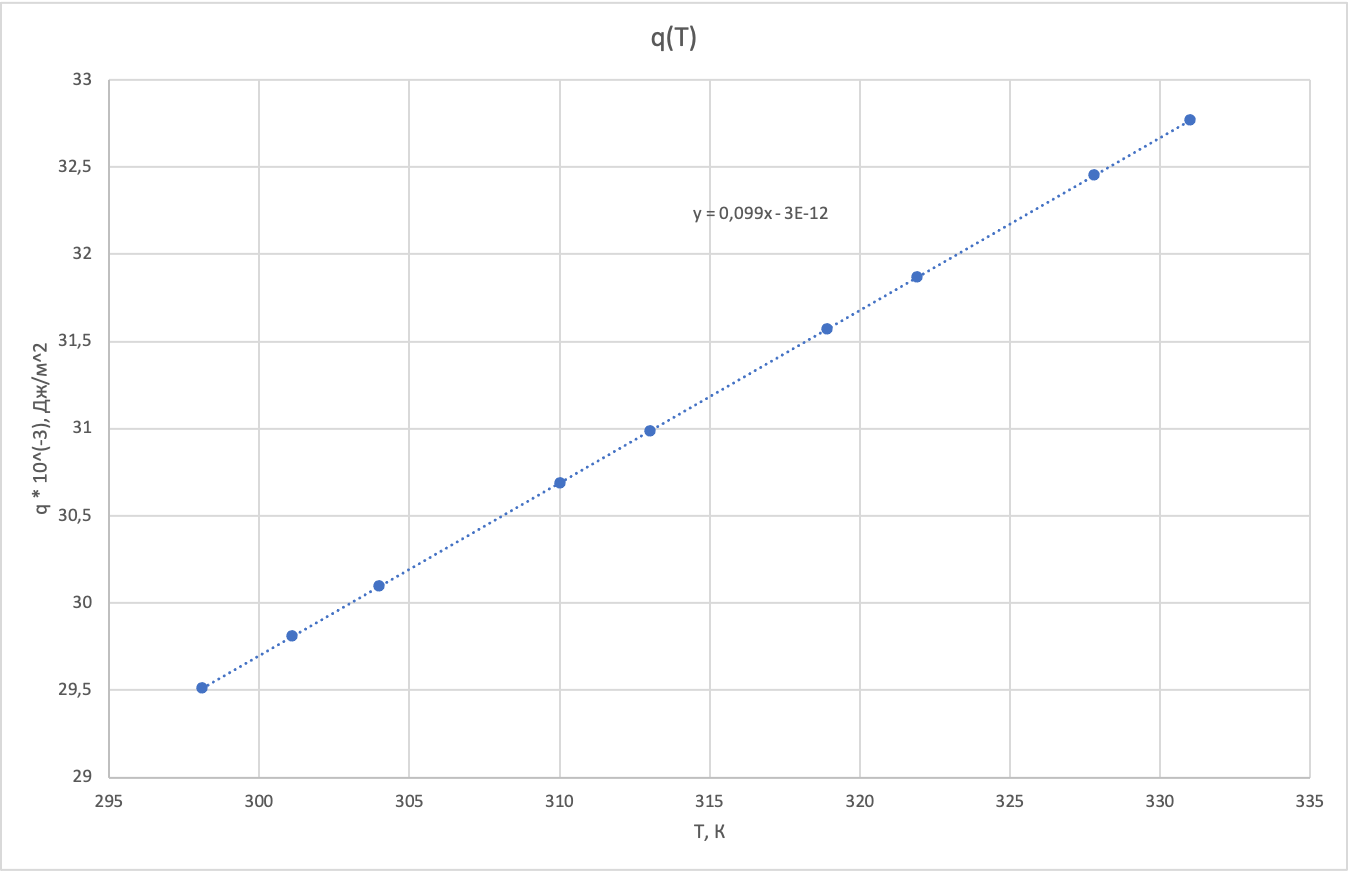
\includegraphics[width=0.75\linewidth]{images/q(T).png}
            \caption{График зависимости $q(T)$}
            \label{pic3}
        \end{figure}
        
        \begin{figure}[ht]
            \centering
            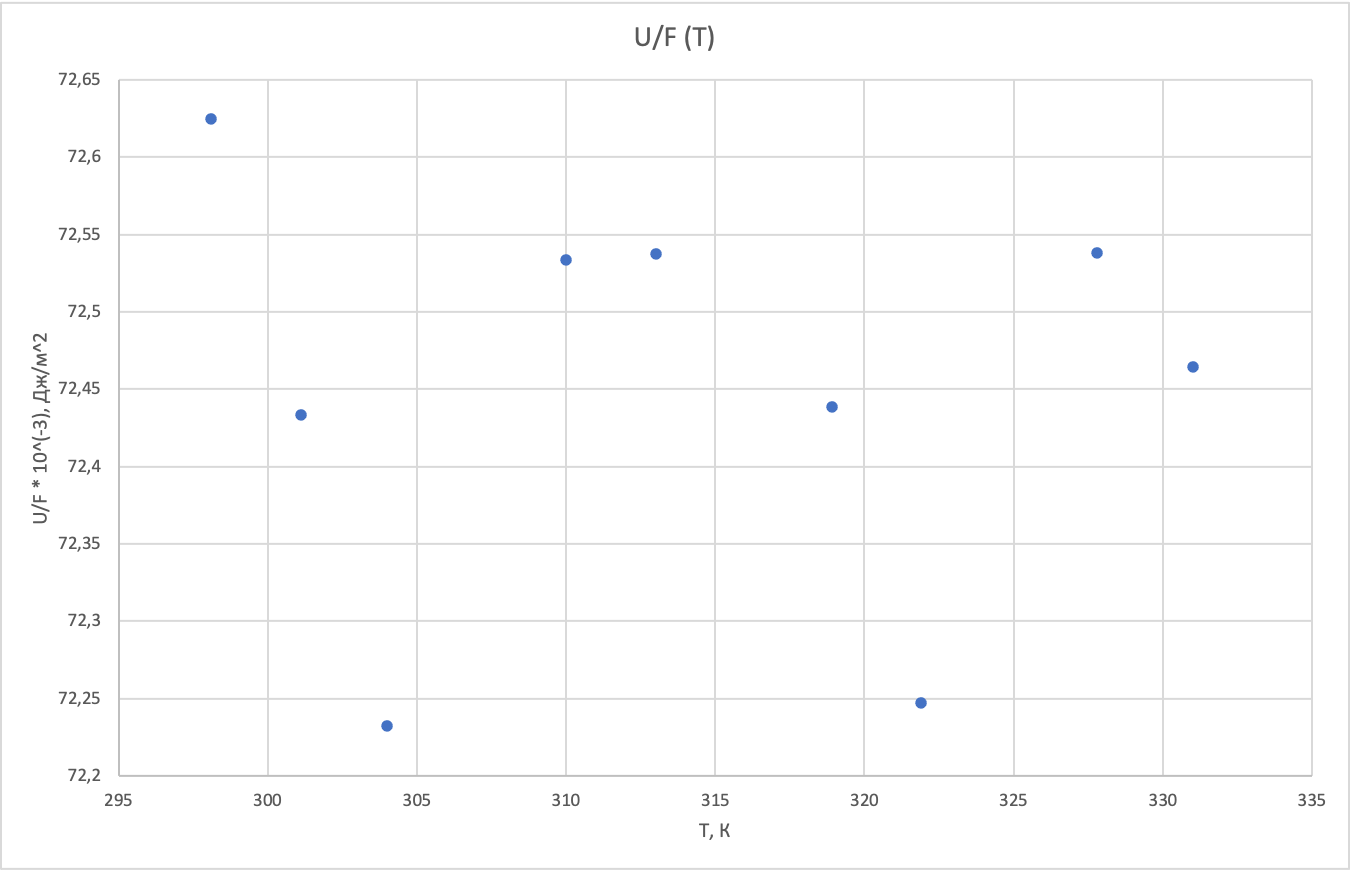
\includegraphics[width=0.75\linewidth]{images/UF_(T).png}
            \caption{График зависимости $\frac{U}{F}(T)$}
            \label{pic4}
        \end{figure}
        
    \end{enumerate}
    
    \newpage
    
    \begin{flushleft}
        {\Large {\bf Вывод}}
    \end{flushleft}
    
    В ходе данной работы была экспериментально проверена формула Лапласа, измерен коэффициент поверхностного натяжения воды, исследована зависимость коэффициента поверхностного натяжения воды от температуры. Также были построены графики зависимости единицы поверхности жидкости от температуры и поверхностной энергии с единицей площади от температуры. Помимо всего мы сравнили косвенные измерения расстояний с их прямыми измерениями, но из-за существенных погрешностей одни совпали с другими только по порядку. Также значение коэффициента поверхностного натяжения воды получилось меньше своего табличного значения. Это может быть связано со множеством факторов. Например в воде мог находиться слой жира от иглы, которую до этого трогали грязными руками. 

\end{document}